\section{Vorbereitung}
\label{sec:preperation}





\section{Analyse}
\label{sec:analyse}




\section{Clustering}
\label{sec:cluster}
\subsection{}
\subsection{}
Spielt man eine Violine mit mehr Dynamik, treten die Obertöne stärker hervor.
Das heißt die harmonischen Frequenzen der Grundfrequenz haben größere Amplituden im Verhältnis zur Grundfrequenz als wenn man den Bogen nur langsam und mit wenig Druck über die Saite streicht.  
Die daraus folgende Änderung in der Gestalt des Frequenzspektrums lässt sich mit den zwei Deskriptoren Spectral Skewness, welche die Asymetrie des Spektrums beschreibt und Spectral Kurtosis, welche die Ähnlichkeit des Spektrums zu einer Gaußkurve beschreibt quantifizieren. 

\subsection{}


\subsection{}

\begin{figure}[H]
    \center
    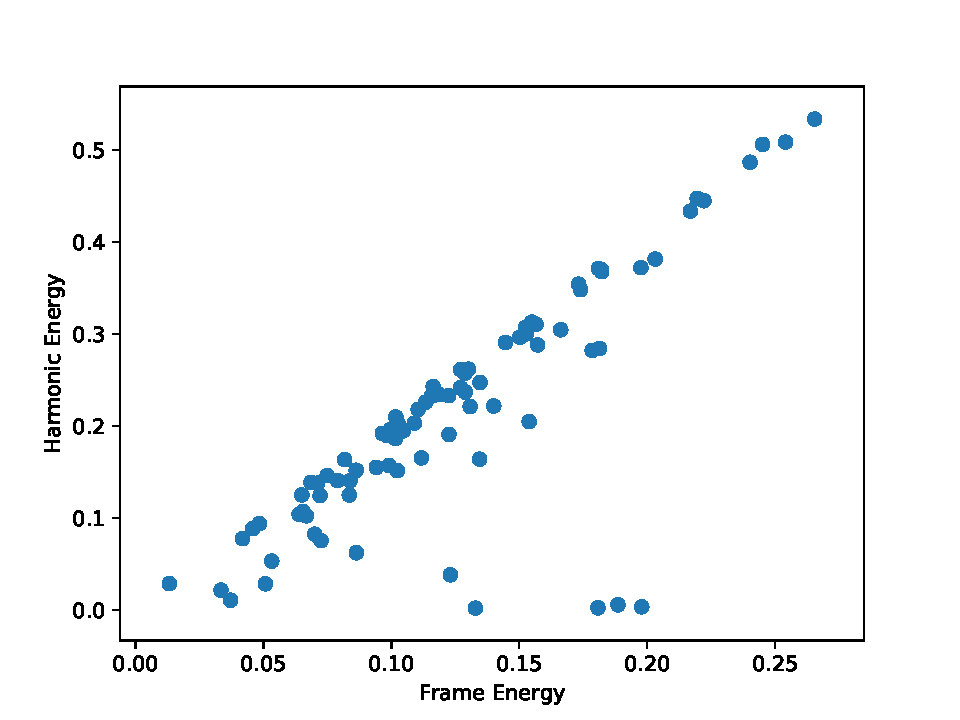
\includegraphics[width = 0.8\textwidth]{Figures/harmonicErg}
    \caption{Harmonic Energy}
    \label{fig:im}
\end{figure}

\begin{figure}[H]
    \center
    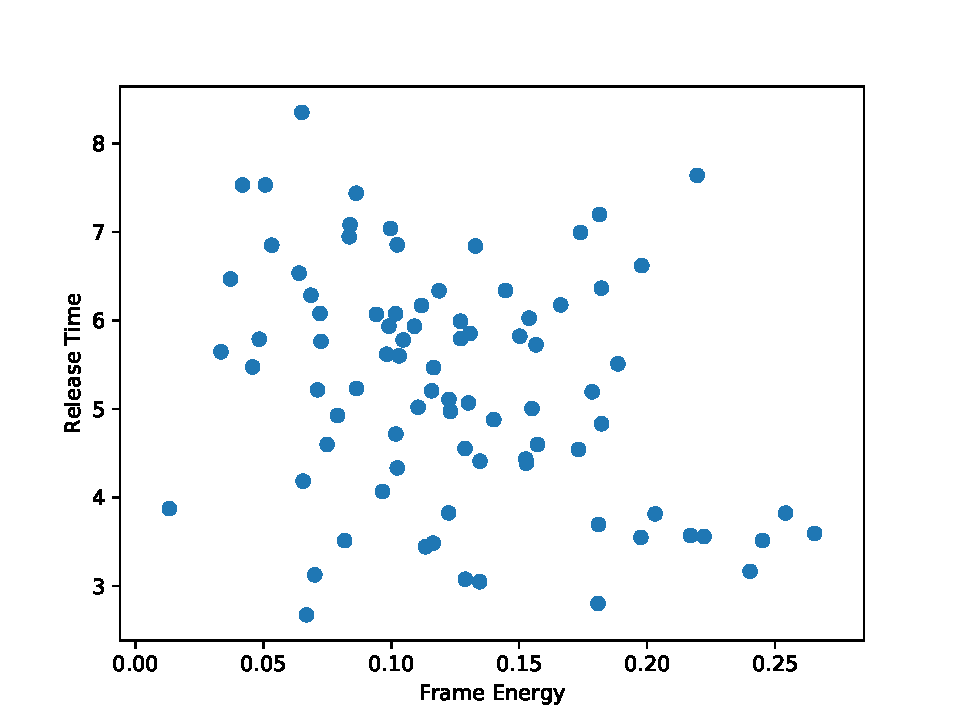
\includegraphics[width = 0.8\textwidth]{Figures/rel.pdf}
    \caption{Release Time}
    \label{fig:im}
\end{figure}

\begin{figure}[H]
    \center
    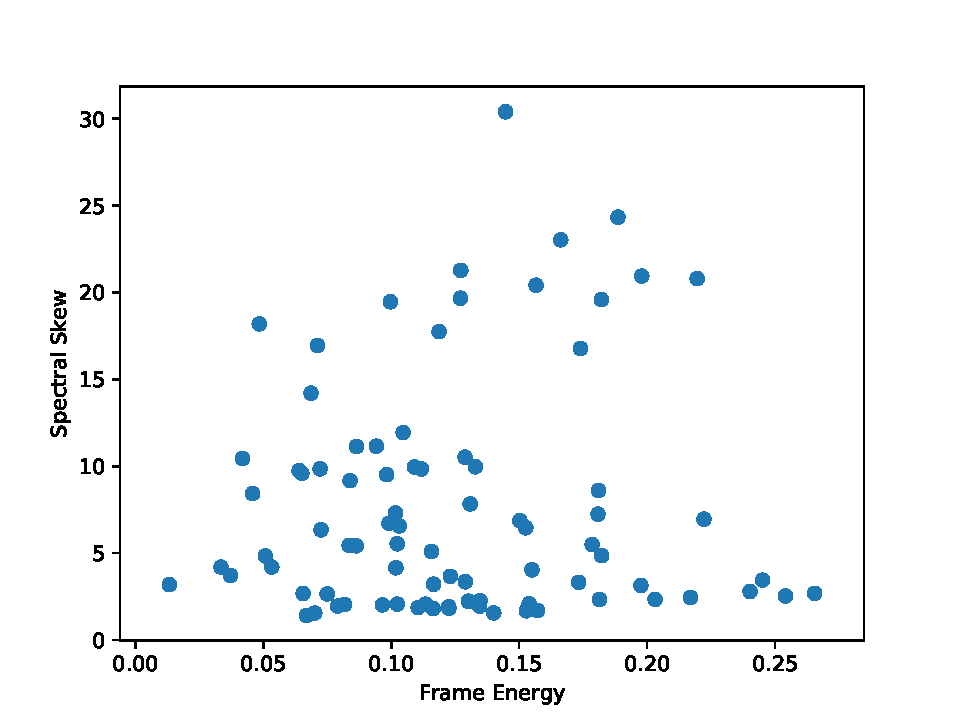
\includegraphics[width = 0.8\textwidth]{Figures/specSkew.pdf}
    \caption{Spectral Skew}
    \label{fig:im}
\end{figure}

\begin{figure}[H]
    \center
    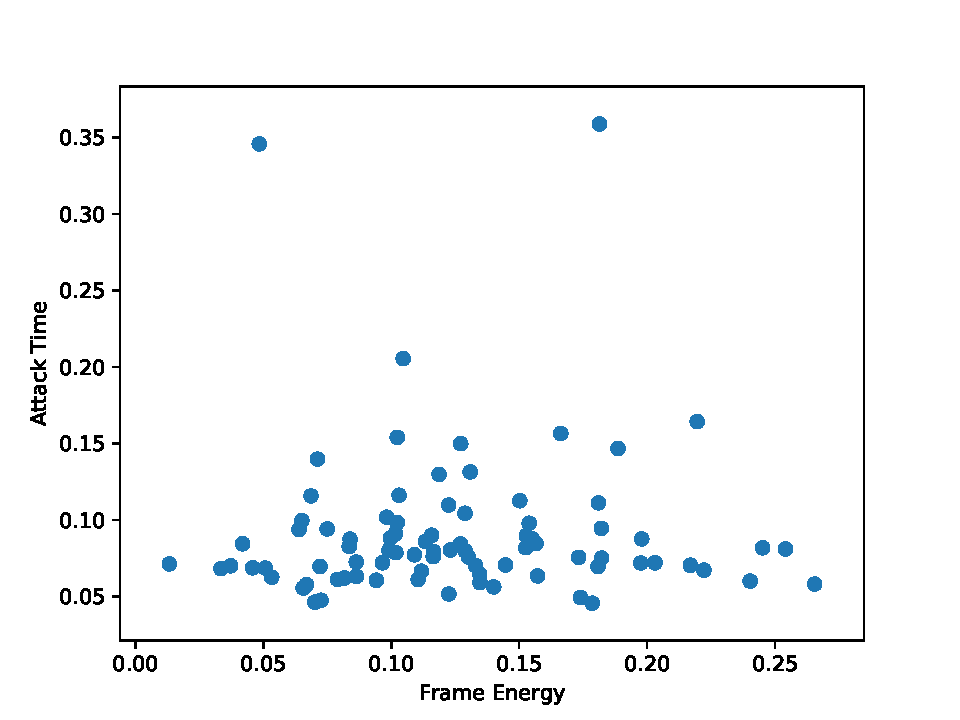
\includegraphics[width = 0.8\textwidth]{Figures/att.pdf}
    \caption{Attack Time}
    \label{fig:im}
\end{figure}